\subsection{Lệnh find}
\underline{\textbf{Chức năng của lệnh:}} Lệnh \verb|find <dir> <fname1> [fname2] ...| được dùng để tìm kiếm các tập tin tên \verb|fname1|, \verb|fname2|... trong thư mục \verb|dir| \cite{mit-xv6}.

\underline{\textbf{Thiết lập thuật toán:}}

Hàm \mintinline{C++}|void find(char* root, char* name)|:
\begin{enumerate}[labelindent=1em, labelsep=0.2cm, leftmargin=1cm, wide=\parindent, topsep=0.1cm, itemsep=-1ex, partopsep=1.5ex, parsep=1.5ex]
	\item Mở đường dẫn của cây thư mục đầu vào, nếu thành công sẽ đọc metadata của cây thư mục đó.
	\item Phân loại các mục có trong thư mục đó, nếu đó là FILE, sẽ tiến hành đối chiếu với tên tập tin cần tìm, nếu đúng sẽ in ra đường dẫn tới tập tin đó, không thì sẽ bỏ qua. Nếu đó là DIR, tiến hành đệ quy đường dẫn tới thư mục đó kèm tên tập tin cần tìm.
	\item Hàm kết thúc khi metadata của cây thư mục đầu vào được đọc hết.
\end{enumerate}

Hàm \verb|main|:
\begin{enumerate}[labelindent=1em, labelsep=0.2cm, leftmargin=1cm, wide=\parindent, topsep=0.1cm, itemsep=-1ex, partopsep=1.5ex, parsep=1.5ex]
	\item Kiểm tra cú pháp của \verb|find|. Lệnh sẽ báo lỗi khi người dùng nhập sai cú pháp.
	\item Thực hiện tìm kiếm với từng tên tập tin có trong câu lệnh.
\end{enumerate}

\underline{\textbf{Khó khăn đã gặp phải:}}
\begin{itemize}[labelindent=1em, labelsep=0.2cm, leftmargin=1cm, wide=\parindent, topsep=0.1cm, itemsep=-1ex, partopsep=1.5ex, parsep=1.5ex]
	\item Hiểu cơ chế đọc metadata của tập tin/thư mục có trong xv6.
	\item Thiết kế giải pháp tránh các lỗi như đệ quy vô hạn khi hàm \verb|find| nhận đầu vào là chính bản thân cây đường dẫn đang được đọc.
\end{itemize}
\newpage
Dưới đây là kết quả chạy thử trên \verb|qemu| và kiểm tra lệnh \verb|find| bằng chương trình kiểm thử:
\begin{figure}[htp!]
	\centering
	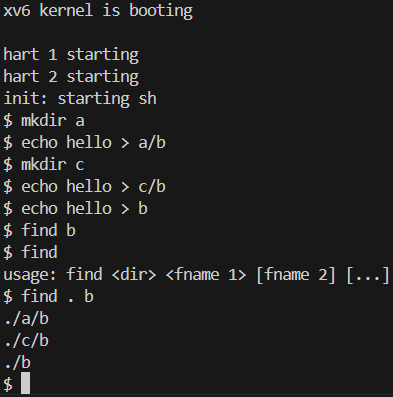
\includegraphics[width=0.5\textwidth]{figures/exec-find}
	\caption{Kết quả chạy thử \textbf{find} trên \textbf{qemu}}
\end{figure}
\begin{figure}[htp!]
	\centering
	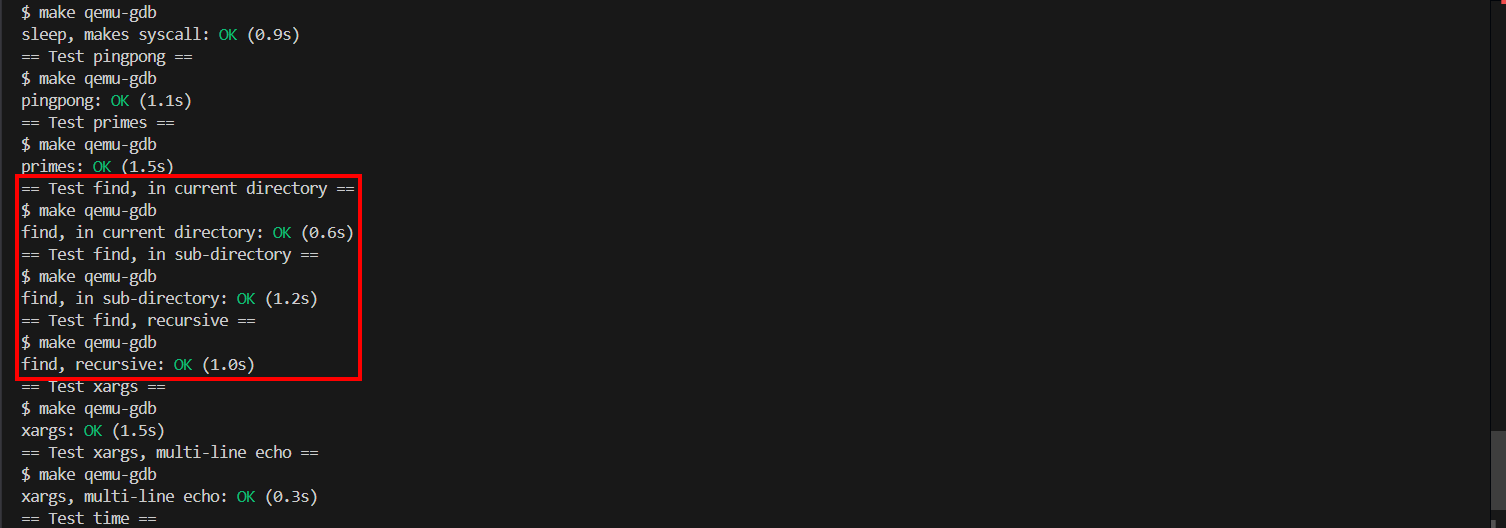
\includegraphics[width=0.9\textwidth]{figures/find-test}
	\caption{Kết quả kiểm thử \textbf{find} bằng công cụ chấm bài \textbf{grade} của MIT}
\end{figure}